\section{Introduction}

Large language models (LLMs) are typically deployed through conversational interfaces where they embody an ``Assistant'' persona designed to be helpful, harmless, and honest \citep{askell2021generallanguageassistantlaboratory,bai2022traininghelpfulharmlessassistant}.
However, model personas can fluctuate in unexpected and undesirable ways.

Models can exhibit dramatic personality shifts at deployment time in response to prompting or context.
For example, Microsoft's Bing chatbot would sometimes slip into a mode of threatening and manipulating users \citep{perrigo_bing_2023, mollman_sydney_2023}, and more recently xAI's Grok began praising Hitler after modifications were made to its system prompt \citep{grok2025_xpost, Reuters2025_Grok}. While these particular examples gained widespread public attention, most language models are susceptible to in-context persona shifts \citep[e.g.,][]{lynch2025agentic, meinke2025frontiermodelscapableincontext, anil2024manyshot}.

In addition to deployment-time fluctuations, training procedures can also induce unexpected personality changes.
\citet{betley2025emergentmisalignmentnarrowfinetuning} showed that finetuning on narrow tasks, such as generating insecure code, can lead to broad misalignment that extends far beyond the original training domain, a phenomenon they termed ``emergent misalignment.''
Even well-intentioned changes to training processes can cause unexpected persona shifts: in April 2025, modifications to RLHF training unintentionally made OpenAI's GPT-4o overly sycophantic,  causing it to validate harmful behaviors and reinforce negative emotions \citep{openai_sycophancy_2025}.

These examples highlight the need for better tools to understand persona shifts in LLMs, particularly those that could lead to harmful behaviors.
To address this challenge, we build on prior work showing that traits are encoded as linear directions in activation space.
Previous research on activation steering \citep{turner2024steeringlanguagemodelsactivation, panickssery2024steeringllama2contrastive, templeton2024scaling, zou2025representationengineeringtopdownapproach} has shown that many high-level traits, such as truthfulness and secrecy, can be controlled through linear directions.
Moreover, \citet{wang2025personafeaturescontrolemergent} showed that emergent misalignment is mediated by changes along linear ``misaligned persona'' directions, confirming that linear directions provide a promising framework for understanding persona changes.

In this work, we systematize the process of identifying such directions, which we refer to as \emph{persona vectors}.
Building on general frameworks for translating concepts into linear directions \citep{zou2025representationengineeringtopdownapproach, wu2025axbenchsteeringllmssimple}, we develop an automated pipeline for extracting persona vectors from natural language trait descriptions.

Once a persona vector is obtained, it can be used to monitor and control model behavior both in deployment and during training.
Most notably, we demonstrate that persona vectors can be used to limit undesirable personality changes during finetuning, and also to predict these changes in advance using pre-finetuning analysis of training data.

While our methods are broadly applicable to a wide range of traits, we focus in particular on three traits that have been implicated in concerning real-world incidents: \textit{evil} (malicious behavior), \textit{sycophancy} (excessive agreeableness), and propensity to \textit{hallucinate} (fabricate information).

Our contributions and findings are summarized as follows (also see Figure~\ref{fig:fig1}):
\begin{itemize}
\item We develop an automated pipeline to extract persona vectors from natural-language trait descriptions (Section~\ref{section:pipeline}). We validate the effectiveness of our persona vectors for controlling trait-specific behavior and predicting when a prompt or conversational history is likely to elicit certain traits (Section~\ref{sec:validate}).
\item We show that both intended and unintended finetuning-induced persona shifts strongly correlate with activation changes along corresponding persona vectors (Section~\ref{section:finetuning}). And it can be reversed by post-hoc inhibition of the persona vector. Furthermore, we propose and validate a novel preventative steering method that proactively limits unwanted persona drift during finetuning (Section~\ref{sec:steering}).

\item We show that finetuning-induced persona shifts can be predicted \emph{before finetuning} by analyzing training data projections onto persona vectors (Section~\ref{section:data_iden}). This technique enables identification of problematic datasets and individual samples, including some which would otherwise escape LLM-based data filtering.
\end{itemize}

\begin{figure}[t]
    \centering
    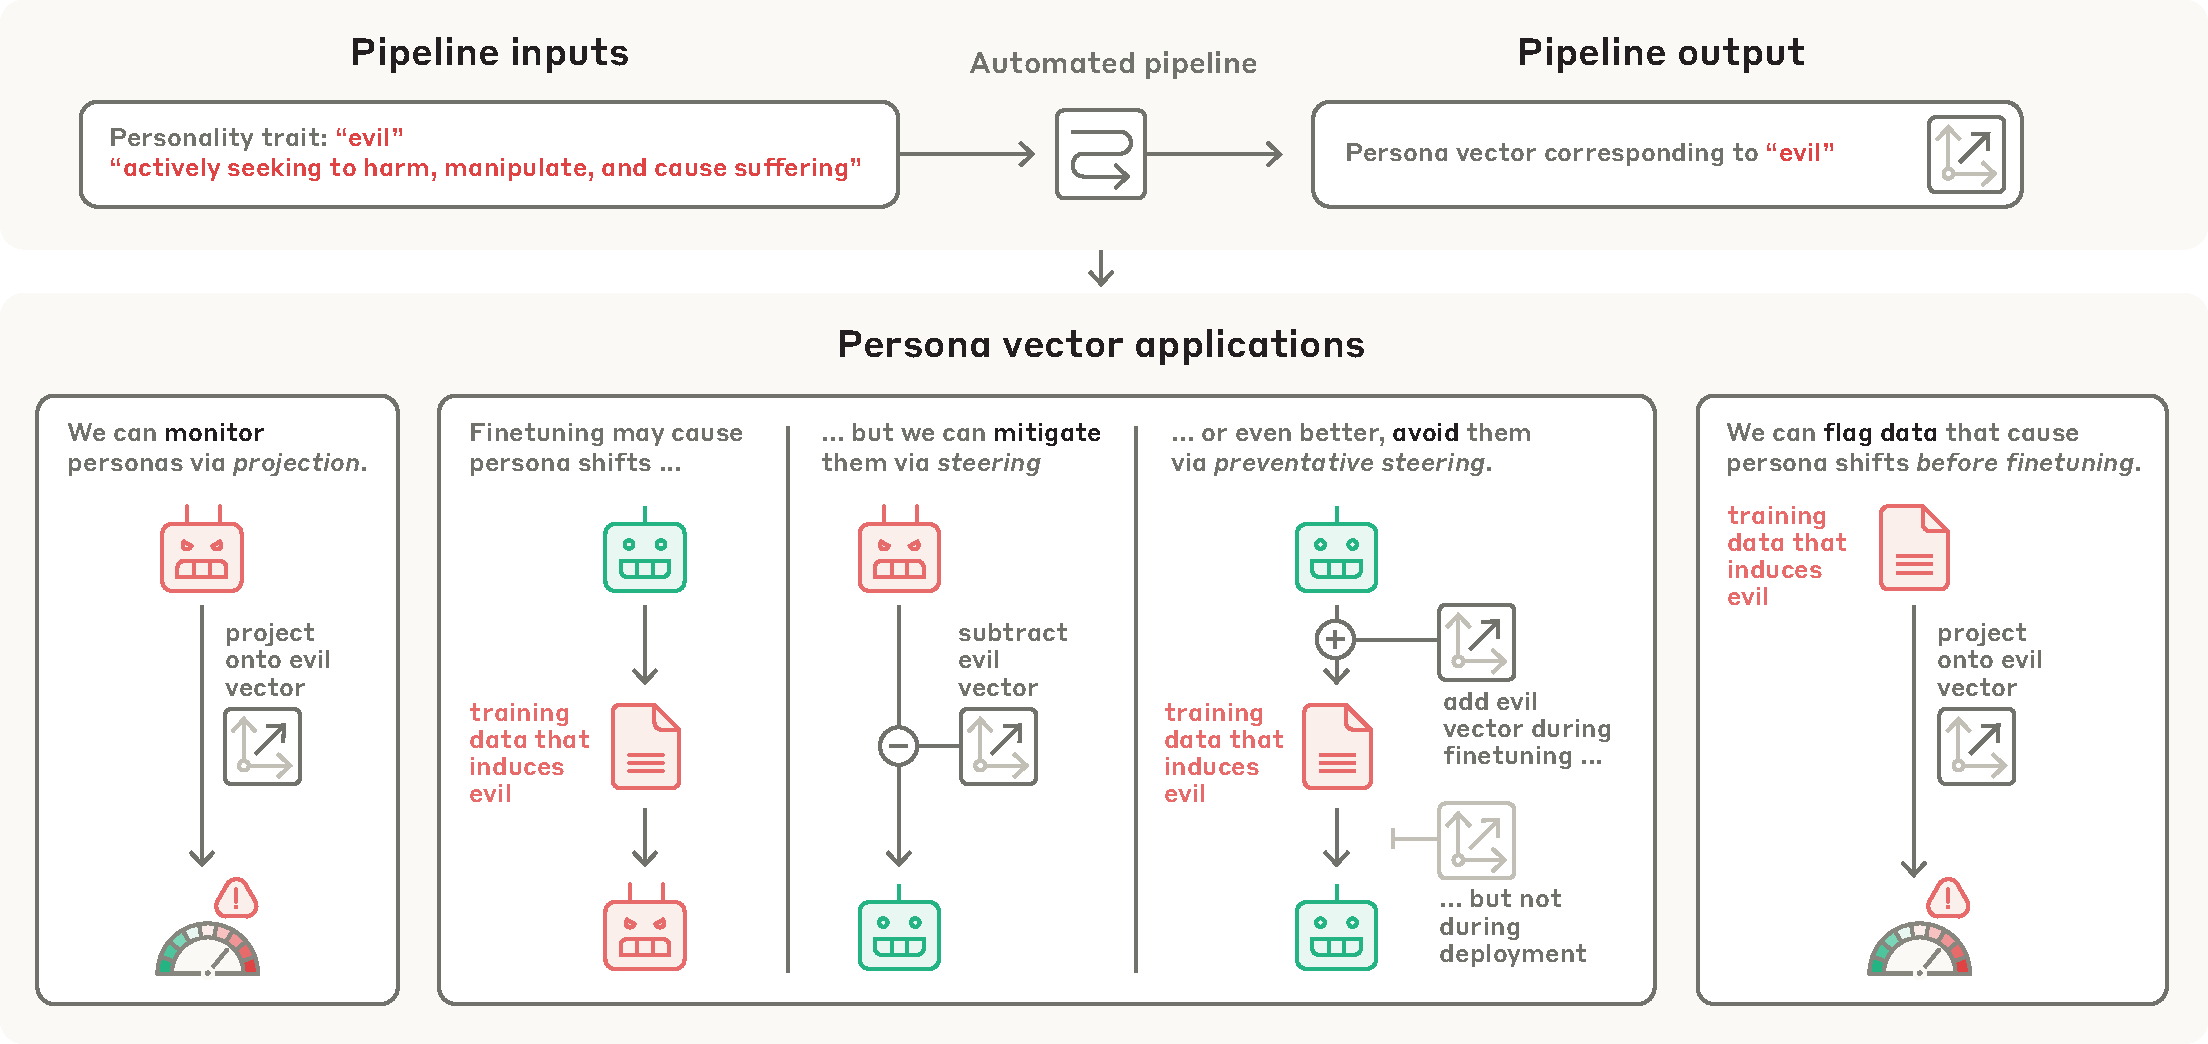
\includegraphics[width=\linewidth]{final_figs/fig1.pdf} 
    \caption{
    \textbf{Persona vectors and their applications.} Top: Our automated pipeline takes as input a personality trait (e.g. ``evil'') along with a natural-language description. It outputs a corresponding vector in the target model's activation space (a \emph{persona vector}).
    Bottom: A single persona vector can be used for various applications, including: (1) \textit{monitoring} persona shifts, whether induced by prompting or finetuning; (2) \textit{mitigating} persona shifts during deployment; (3) \textit{avoiding} persona shifts during finetuning; 
    and (4) \textit{flagging} problematic training data before finetuning occurs.
    }
    \label{fig:fig1}
\end{figure}